\documentclass[a4paper]{article}
\usepackage{booktabs}
\usepackage{caption}
\usepackage{subcaption}
\usepackage{amsmath}
\usepackage{amsfonts}
\usepackage{amssymb}
\usepackage{lscape}
\usepackage{psfrag}
\usepackage[usenames]{color}
\usepackage{bbm}
\usepackage[update]{epstopdf}
\usepackage[bookmarks,pdfstartview=FitH,pdfborder={0 0 0}]{hyperref}
\usepackage{verbatim}
\usepackage{listings}
\usepackage{textcomp}
% \usepackage{course}
\usepackage{fancyhdr}
\usepackage{multirow}
\usepackage[demo]{graphicx}
% \pagestyle{fancy}
\usepackage{tikz}

\usepackage[utf8]{inputenc}
\usepackage[english]{babel}
%Image-related packages
\usepackage[export]{adjustbox}
\usepackage{wrapfig, , csquotes}
% \usepackage[
% backend=biber,
% style=alphabetic,
% sorting=ynt
% ]{biblatex}
%------------------------------

\renewcommand{\sectionmark}[1]{\markboth{#1}{#1}}
\renewcommand{\subsectionmark}[1]{\markright{#1}}

% \fancyhf{}
% \fancyhead[RO]{\nouppercase{\footnotesize\sc\leftmark\ \hrulefill\ \thepage}}
% \fancyhead[RE]{\nouppercase{\footnotesize\sc\thepage\ \hrulefill\ }}
% \renewcommand{\headrulewidth}{0pt}

\makeatletter
\def\cleardoublepage{\clearpage\if@twoside \ifodd\c@page\else%
\hbox{}%
\thispagestyle{empty}%
\clearpage%
\if@twocolumn\hbox{}\clearpage\fi\fi\fi}
\makeatother


\renewcommand{\topfraction}{0.9}  % max fraction of floats at top
\renewcommand{\bottomfraction}{0.8} % max fraction of floats at bottom
% Parameters for TEXT pages (not float pages):
\setcounter{topnumber}{2}
\setcounter{bottomnumber}{2}
\setcounter{totalnumber}{4}            % 2 may work better
\setcounter{dbltopnumber}{2}           % for 2-column pages
\renewcommand{\dbltopfraction}{0.9}    % fit big float above 2-col. text
\renewcommand{\textfraction}{0.07}     % allow minimal text w. figs
% Parameters for FLOAT pages (not text pages):
\renewcommand{\floatpagefraction}{0.7}  % require fuller float pages
% N.B.: floatpagefraction MUST be less than topfraction !!
\renewcommand{\dblfloatpagefraction}{0.7} % require fuller float pages


\edef\today{%\number\day\
\ifcase\month\or
January\or February\or March\or April\or May\or June\or July\or
August\or September\or October\or November\or December\fi\ \number\year}
\title{\vspace*{40.0mm}
    \bf Computer Vision Report\\Incisor Segmentation
    \vspace*{20.0mm} \\
    \vspace*{40.0mm}
    %\vspace{-20mm}\framebox{DRAFT VERSION}\vspace{20mm} \\
    %\Large\bf Support Vector Machines Assignment
\author{
    \Large Orsolya Lukacs-Kisbandi, r0650042 \\
    \Large Stefano Proto, r065080}
}

\begin{document}

\begin{figure}
    \parbox[t]{125mm}{
        \vspace*{6mm}
        \scriptsize\sf           FACULTY OF ENGINEERING SCIENCE\\
        \scriptsize\sf           PROGRAMME FOR EXCHANGE STUDENTS \\
        \scriptsize\sf\bfseries  COMPUTER SCIENCE \\
        \scriptsize\sf           KASTEELPARK ARENBERG 40 B-3001 LEUVEN}
        \parbox[t]{40mm}{
        \begin{flushright}
            
\includegraphics[height=15mm]{logokul.pdf}
        \end{flushright} }
\end{figure}

\maketitle
\thispagestyle{empty}
\raggedbottom

\cleardoublepage
\setcounter{tocdepth}{2}
\cleardoublepage
\pagenumbering{arabic}

\maketitle
\thispagestyle{empty}
\newpage
\tableofcontents
\thispagestyle{empty}
\newpage
\setcounter{page}{1}

\section{Introduction}
The aim of this project was to write an algorithm that is capable of segmenting the upper and lower incisors in panoramic radiographs using a model based approach.
The chosen method is called Active Shape Models, and it is described in \cite{cootes} Cootes at al. The implemented algorithm can be broken down into sub-parts, namely: building the Active Shape Model, described in section \ref{sec:modelling}, pre-processing the input images, explained in section \ref{sec:preprocessing}, and finally fitting the model on the images, as presented in section \ref{sec:fitting}. In addition, our observations and experimental results will be discussed in the final part of the report. 

\section{Active Shape Model}\label{sec:modelling}
The reason for building Active Shape Models for every incisor is to create a general representation of each one of them. By obtaining these models from combining different variations of the same tooth extracted from different peoples' readiographs, we can build a global model which can be fit on the same incisor for new images. This is a good approach four such problems because it creates a general representation of the object in interest, becoming more robust against variability.

Active Shape Models are based on a prior model of what is expected to be seen on the new image. In our case these are the incisors, represented by a set of characteristic points, the landmarks. Based on these landmarks, a general model of the expected shape is created, which can be used to find the best match of the model in the new image. This model gives a compact representation of the previous knowledge allowing some variation, but being specific enough to exclude changes which haven't been seen in the training data. The landmarks are specific coordinates on the training images which represent a distinguishable point which appears on every training example.

\subsection{Mean shape} 
The training set contains samples from several people. For each person in the training data, every incisor is represented by a set of 40 landmark points describing the shape of the tooth. In order to create the models, the shape of each tooth had to be scaled and translated to the origin, to make the computations easier and for the comparison of landmarks to be possible. Translating the images also included rotating them by an angle $\theta$ so their \textit{x} and \textit{y} axes would be aligned. After the shapes were centered to the origin based on their center of gravity, the scaled mean shape for each tooth was computed. This was necessary because we wanted to build a scale and rotation invariant model which could handle any type of input. \\ 
The following procedure was done iteratively until the mean shapes converged to a value which did not change after realigning the landmarks to the new mean as proposed in \cite{cootes2}. After obtaining the mean shape, the landmarks were scaled and centered again around the new mean shape. This technique is called the Generalized Procrustes Analysis. The main idea is that the alignment and re-centering of the shapes is done iteratively until the model converges to a value which does not change after adding another iteration. Our models were considered stable when the squared sum of the distance of each shape to the mean was less than $10^{-10}$.\\ The used approach is shown in Figure \ref{fig:procrustes}, while the final result of the computed models can be observed, for each tooth, in Figure \ref{fig:models}.

\begin{figure}[h] 
    \centering
    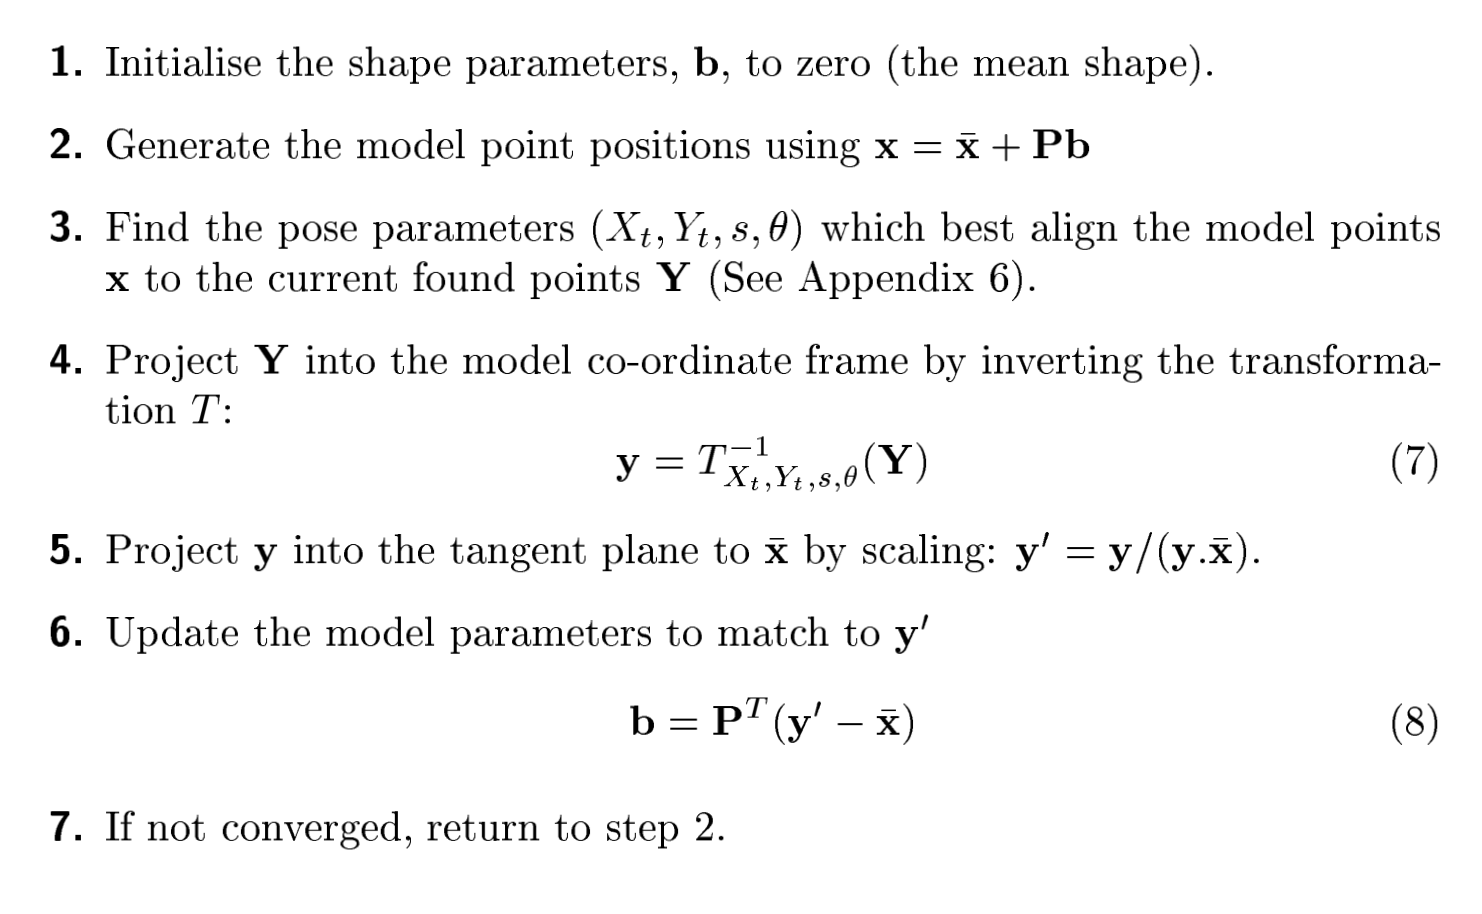
\includegraphics[width=10cm]{asm}
    \caption{Followed procedure to create mean shape models, based on \cite{cootes2}}
    \label{fig:procrustes}
\end{figure}

% \subsection{Principle Component Analysis}
% Principal Component Analysis is a statistical procedure used for identifying a smaller number of uncorrelated variables, called "principal components" from a large set of data to explain the maximum amount of variance with the fewest number of principal components. In other words, the aim of PCA is to reduce the dimensionality of the data. This is an improvement both in terms of memory and computational power.\\
% In our case, we set the number of principal components to 8, which covers 99\% of the variance of the data. This way, we reduced the number of landmarks with a significant amount.

\begin{figure}[h] 
    \centering
    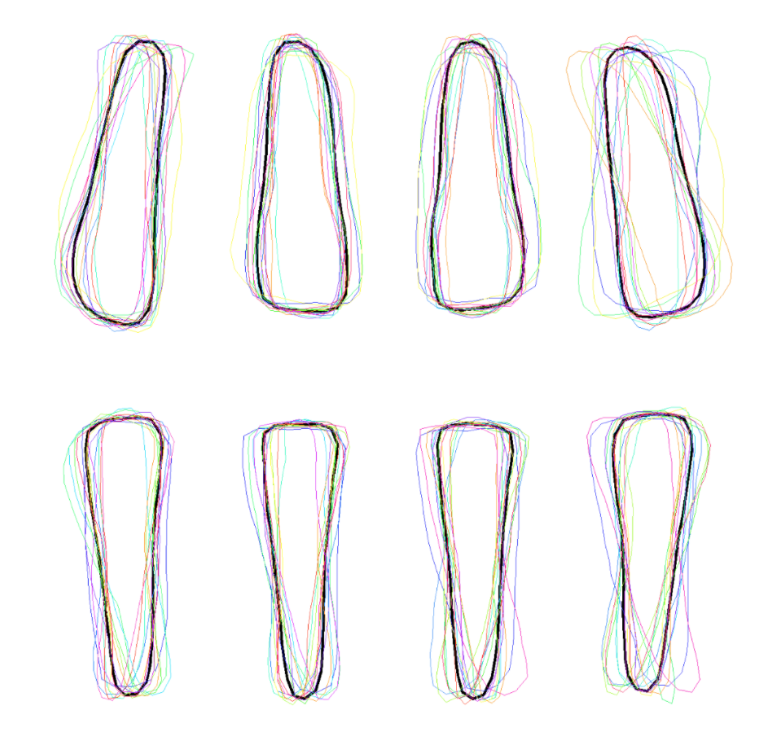
\includegraphics[width=10cm]{activeshapemodel}
    \caption{Final results of the Active Shape Models(black) from the given landmarks (other colors)}
    \label{fig:models}
\end{figure}

\section{Image Processing}\label{sec:preprocessing}
\subsection{Pre-processing}
Radiographs are usually noisy and low in contrast. These characteristics make the image features difficult to extract. In order to overcome this issue, sharpening techniques and contrast enhancement algorithms are applied to the images before they were analyzed. \\
In order to reduce noise, we experimented with different filters, each having it's own advantages and disadvantages. A balance between these filters had to be found, since some of them removed important image features, such as edges and high contrast points. For reducing the impulsive and the Gaussian noise without affecting the edges, a median filter and a bilateral filter was applied.\\
The median filter considers each pixel in the image in turn and looks at the nearby pixels to decide whether or not it is representative of its surroundings. It replaces the pixel value with the median of the neighbouring pixel values. The median is calculated by first sorting all the pixel values from the surrounding neighbourhood into numerical order and then replacing the pixel being considered with the middle pixel value.  Instead of the simple median filter, we tried to apply an adaptive median filter but this required too much computational power as well as time, so we decided to use the much simpler version instead. \\
The Bilateral filter is a non-linear, edge-preserving and noise-reducing smoothing filter. The intensity value at each pixel in an image is replaced by a weighted average of intensity values from nearby pixels, which is based on a Gaussian distribution. Its formulation is simple: each pixel is replaced by an average of its neighbours. It depends only on two parameters that indicate the size and contrast of the features to preserve \cite{paris}. \\ 
The results of the noise suppression can be seen in Step 1 and Step 2 of the preprocessing stages, presented in Figure \ref{fig:preproc}. 
\begin{figure}[h] 
    \centering
    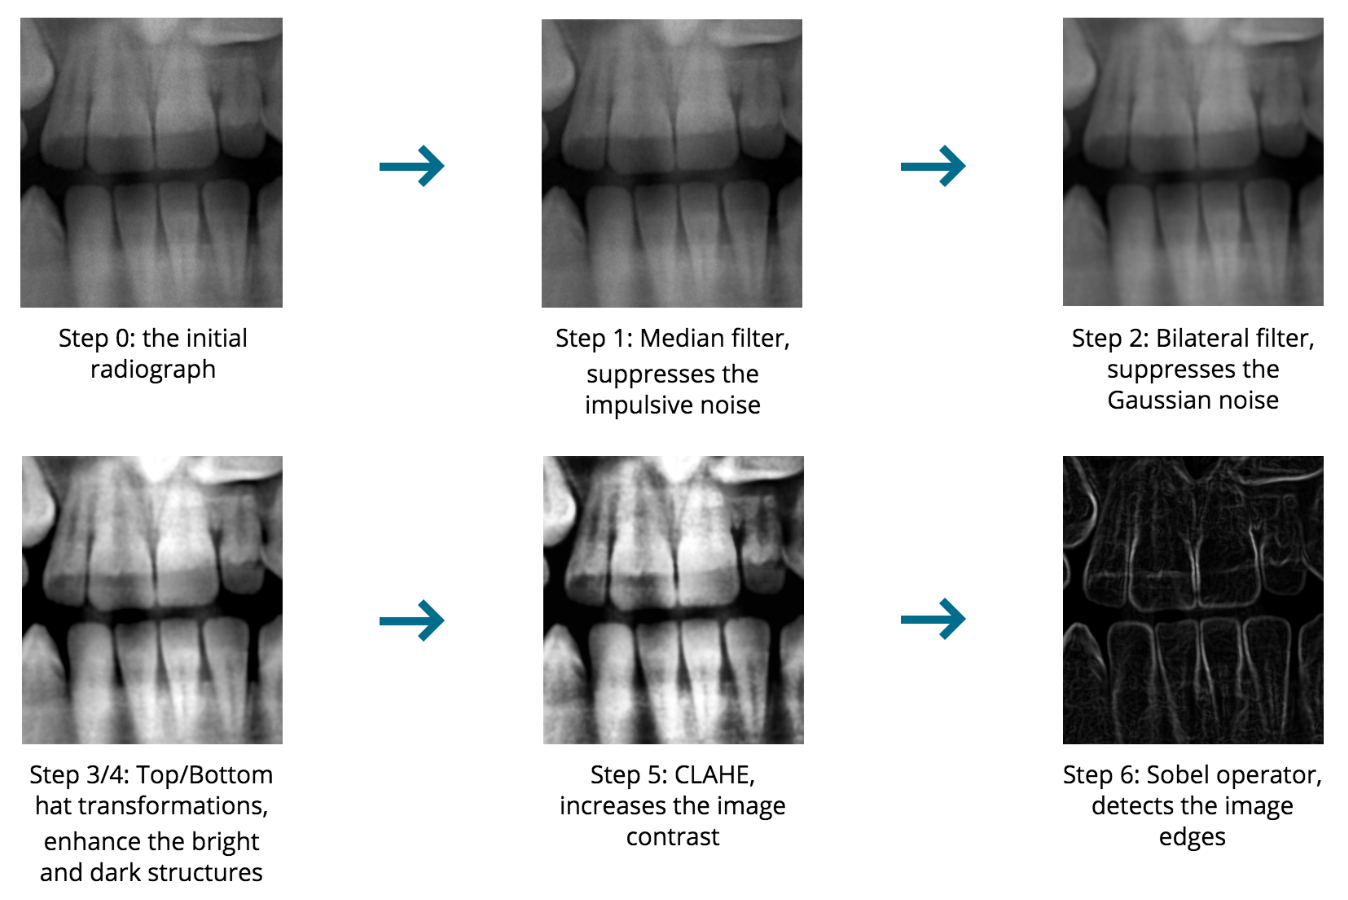
\includegraphics[width=12cm]{preprocessing}
    \caption{Preprocessing stages}
    \label{fig:preproc}
\end{figure}

After these transformations, as suggested in \cite{huang}, the contrast of the image is enhanced by means of two gray-level morphology techniques (top-hat and bottom-hat transform) and a histogram equalization technique. \\
The top-hat transform is able to enhance brighter structures, while the bottom-hat transform enhances the darker structures. The obtained picture from top hat transform is added to, from the bottom hat transform is subtracted from the initial radiograph to apply the effect of this transformations. \\
The last step to enhance the contrast of the image is histogram equalization. For this purpose many approaches were tried: among all the candidate algorithms, in Ahmad et al. \cite{ahmad} it is shown that the Contrast Limited Adaptive Histogram Equalization (CLAHE) better enhances the image quality and increases the diagnostic ease, over performing both the Sharp Contrast Limited Adaptive Histogram Equalization (SCLAHE) and the Median Adaptive Histogram Equalization (SMAHE) \cite{ahmad}.
CLAHE is an improved version of Adaptive Histogram Equalization (AHE). The image is divided into small blocks, and then the histograms are equalized. An important improvement compared to AHE is that, instead of global histogram equalization, the algorithm adapts to local variations in an image, such as shadows and highlights. AHE could amplify the noise, to prevent this, the Contrast Limited technique is used: if any histogram bin is above a specified contrast limit, those pixels are clipped and distributed uniformly to other bins before applying histogram equalization. \\
Steps 3, 4 and 5 presented in Figure \ref{fig:preproc} show the effects of the transforms over the images. 

\subsection{Detecting edges}
In order to find the edges over the images, the Sobel operator is used. The Sobel operator performs a 2-D spatial gradient measurement on an image and emphasizes regions of high spatial frequency that correspond to edges. Typically it is used to find the approximate absolute gradient magnitude at each point in an input grayscale image. \textit{$G_x$} is representing the horizontal changes \textit{$G_y$} the vertical ones on the image.

\[
  G_x=
  \begin{bmatrix}
    -1 & 0 & +1 \\
    -2 & 0 & +2 \\
    -1 & 0 & +1
  \end{bmatrix} * I\quad
  G_y=
  \begin{bmatrix}
    -1 & 2 & -1 \\
    0 & 0 & 0 \\
    +1 & +2 & +1
  \end{bmatrix} * I
\]

At each point of the image we calculate an approximation of the gradient in that point by combining both results above with the following formula.

\begin{align}
   G = \sqrt{ G_x^2 + G_y^2 }
\end{align}

The result of the Sobel operator can be seen at Step 6 of Figure \ref{fig:preproc}. 

\section{Fit model on an image}\label{sec:fitting}
Fitting the models on the image consists of multiple stages. At first hand drawn boxes have to be created to train the system, than the \textit{estimate} function automatically fine tunes them based on the main features of the segment of interest. After returning these boxes, the Active Shape Models are fitted on the image.

\subsection{Hand draw boxes}
In the training part, the user is asked to draw boxes around the upper and lower incisors for every sample image in the training set.\\ 
The obtained boxes are stored in a file, and they are used as initial values for the automatic estimate. For testing, we select the coordinates which are the most extreme, the combination of these representing the largest box, in which all upper or lower incisors will fit in. \\ 
These two boxes (one for the upper and one for the lower incisors) are used as initial estimates on the location of incisors when we are applying our model on an unseen radiograph. Choosing the largest boxes allows the system to be general and include all the teeth, even for unseen images. This assumption was made based on the fact that, when radiographs are taken, the persons' head is facing forward, having the incisors in the middle of the image.  

\subsection{Fine-tune boxes}

\begin{figure}[htp] 
    \centering
    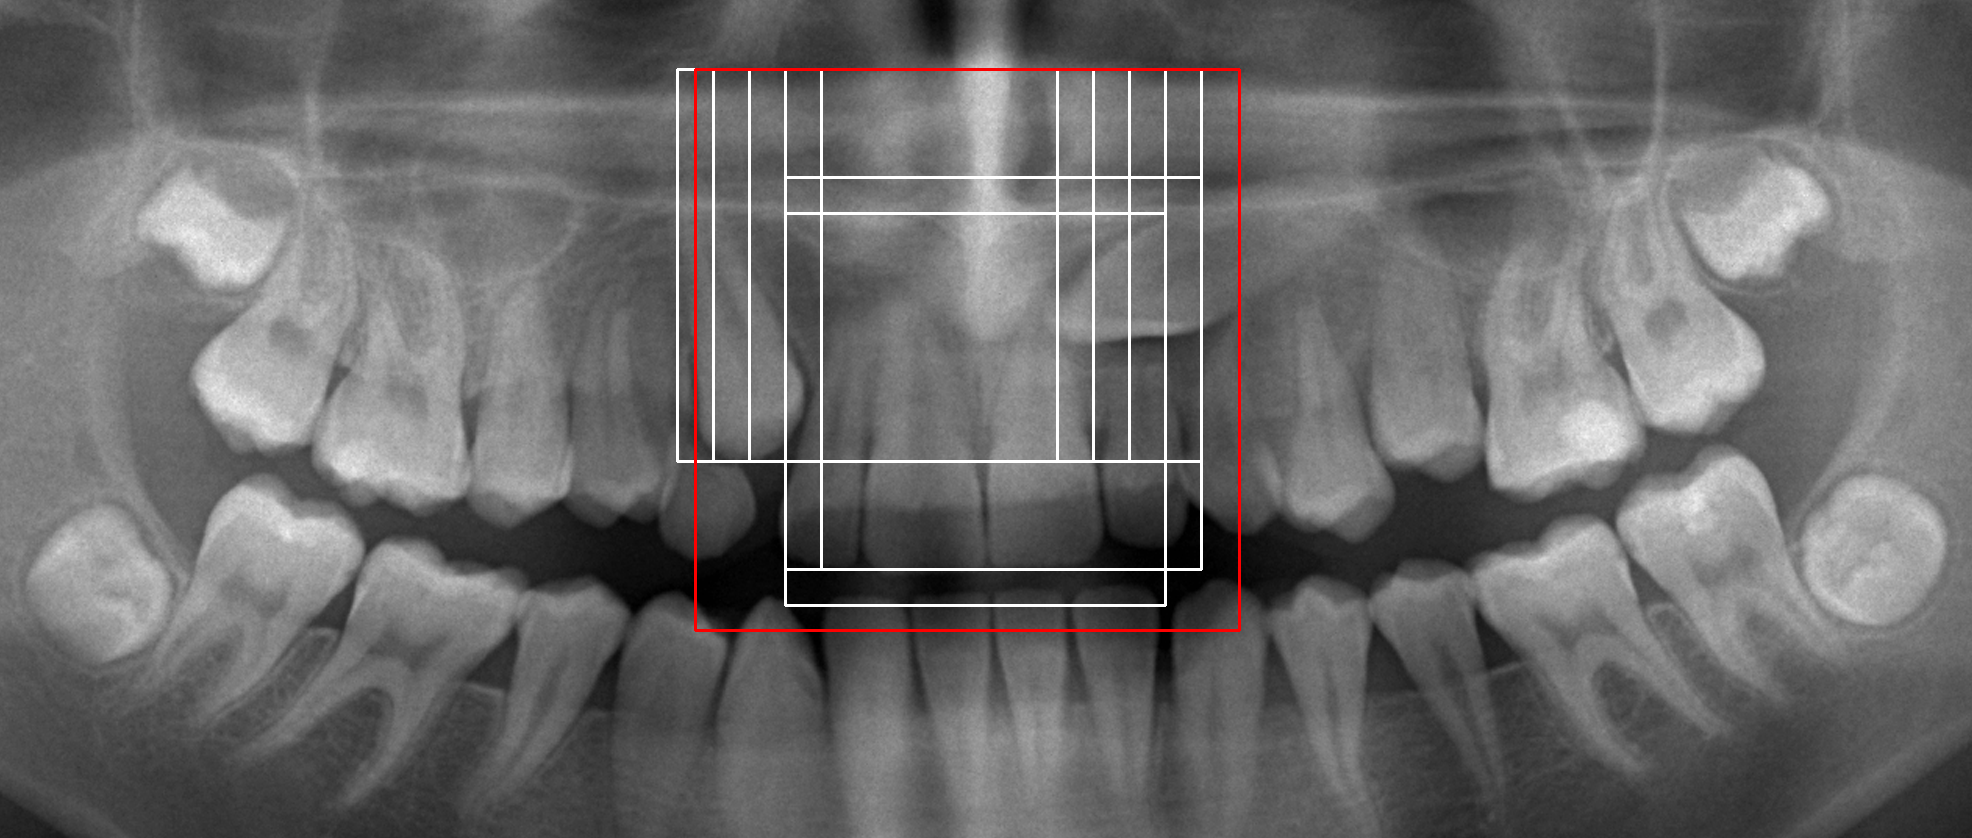
\includegraphics[width=12cm]{sliding2}
    \caption{Windows of different scales (white), sliding over the largest box, searching area, which is marked in red }
    \label{fig:sliding}
\end{figure}

For fine-tuning the boxes the function \textit{estimate} was used. This function takes as parameter a preprocessed radiograph we want to fit the box on, a boolean variable, weather we are looking for an upper or lower incisor, the "biggest box" coordinates, which represent the biggest image segment selected from the hand-drawn boxes, the coordinates from the hand drawn boxes for the particular region and finally \textit{b\_model}, whether we want to build the model or just load the pre-trained model. Using the largest box, the radiographs are cut, resized and flattened (create a N x 1 array from the image segment) based on these coordinates. We apply PCA on the cut images and take the top ten components, which capture most of the variance in the data. After these steps, we invoke the function \textit{best\_seg} which is taking as parameters the mean returned from PCA, the eigenvectors, the bounding box coordinates, the preprocessed radiograph, and the width and height of the box.

In this function, sliding windows of different scales are shifted over the region of interest on the radiograph and the error of reconstructing the segment using the eigenvectors and mean acquired from the cut shapes is calculated. Figure \ref{fig:sliding} shows the windows of different sizes and scales sliding over the searching area. When a window is able to reconstruct the image with a better error, its coordinates are saved. The segment with the smallest error is assumed to be the one better representing the incisor patterns, so it is the one chosen to be returned.  
\\ The result of the box tuning is shown in Figure \ref{fig:bestboxes}: the upper and lower incisors are identified respectively by the two boxes. 

\begin{figure}[h] 
    \centering
    \subcaptionbox{Best box for upper incisor
    \label{cw_10}}{%
        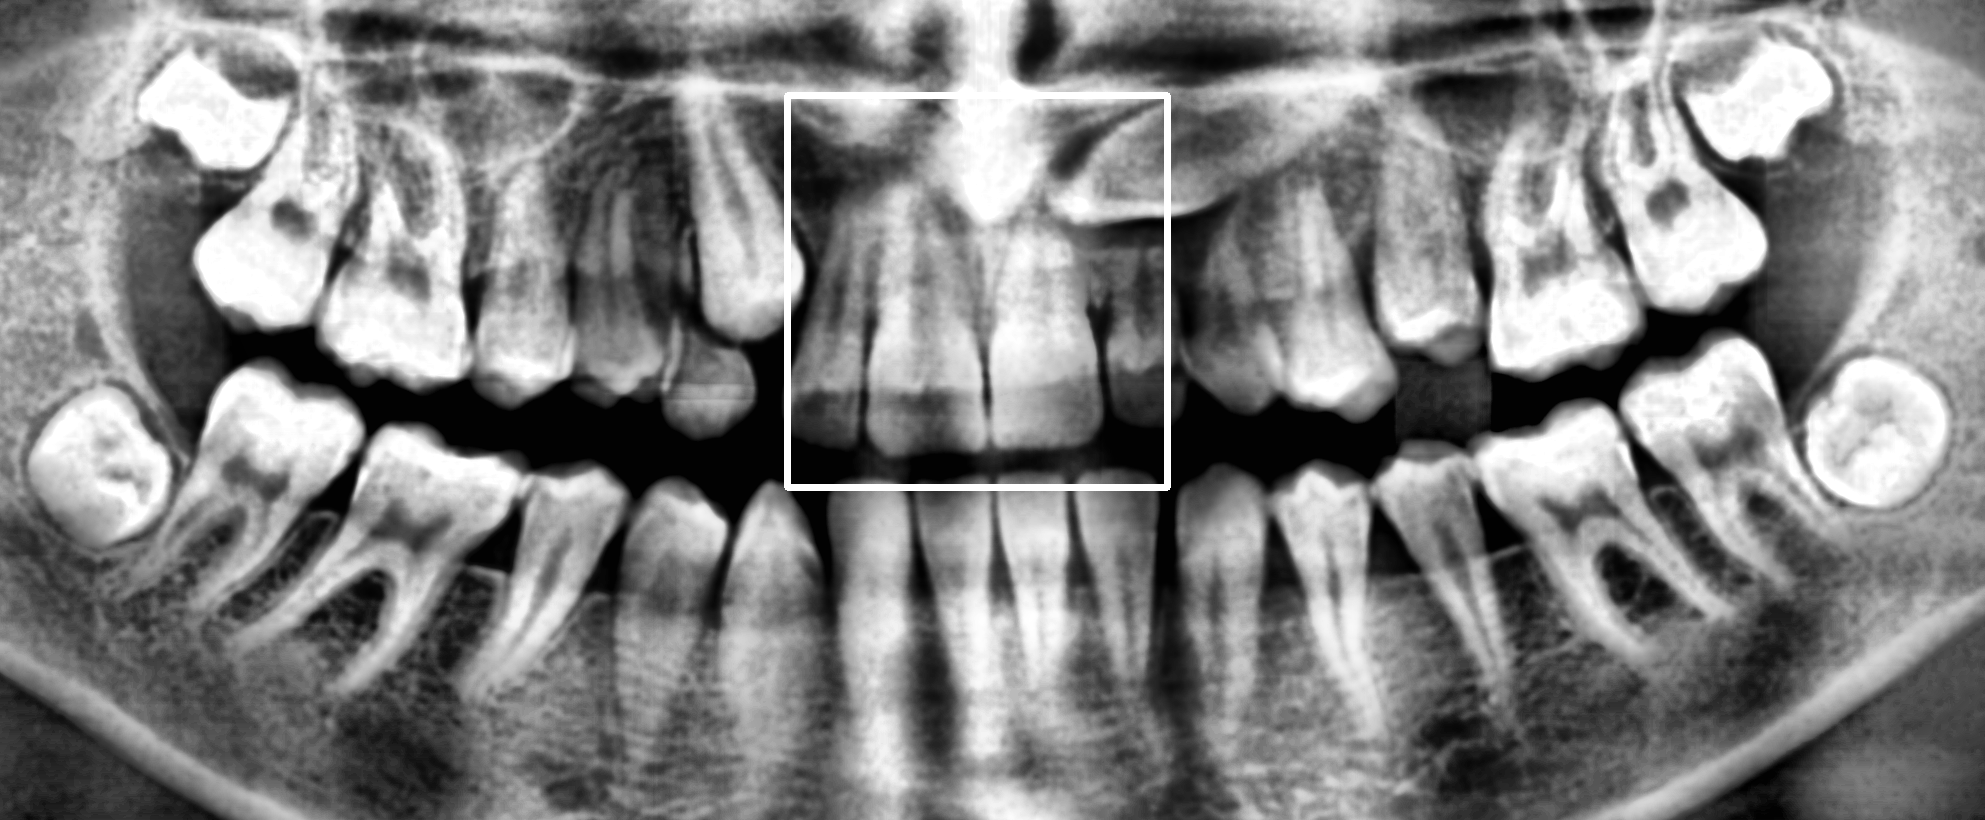
\includegraphics[width=0.8\textwidth]{boxupper00}%
    }\par\medskip
    \subcaptionbox{Best box for lower incisor
    \label{cw_25}}{%
        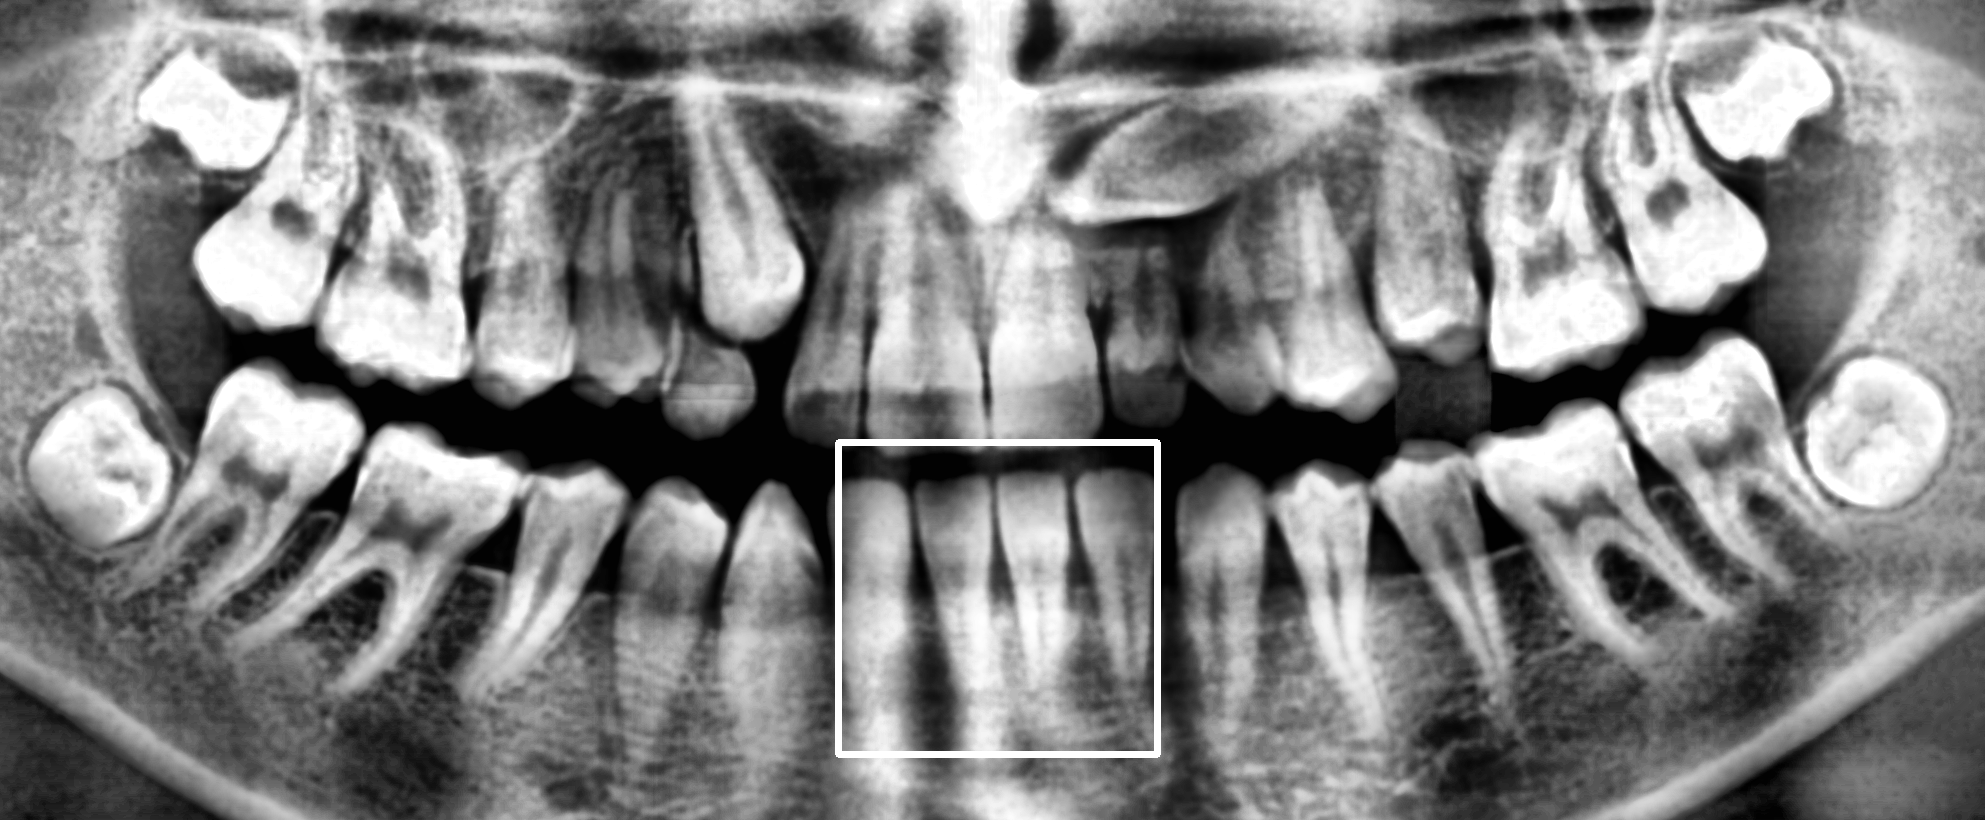
\includegraphics[width=0.8\textwidth]{boxlower00}%
    }\par\medskip        
    \caption{Fitted boxes for Radiograph 0}
    \label{fig:bestboxes}
\end{figure}

\subsection{Fitting the Active Shape Models}
To fit the models, first the upper and lower incisor boxes are divided in four equal parts. This decision is based on the assumption that incisors in the same jaw generally have the same width. Following this, each tooth model is shaped in the corresponding box: the models are centred in the respective tooth box, scaled to fit in it and then centered again. 

After this initial positioning and scaling of the models, they are parsed in order to look for a better estimation of the tooth in their neighbourhood. For every point in the model, the normal line is computed. In case another point is a better fit than the current one, we update the model. The criteria for a point to be better than another is to have a higher value, since edges are represented by light regions. For this reason, brightness along the norm to the model at the current point is compared with the current value of the model on this line. 
\\ In order to have a greater resistance to noise not only the points on the line are considered, but for each point all its neighbours are evaluated. An average of the region is computed, and then compared with the current brightest point for the line: if the value of the region is greater than a certain threshold (directly depending on the current brightest point), then the centre of the evaluated region will become part of the model. The parameters that allow flexibility in the model are the length of the norm we calculate (this can decide on the region we are looking for points which are more likely to be edges) the step we traverse the shape of the incisor, larger step is more resistant to noise, while smaller steps are following the shape more precisely. \\
The chosen values for the parameters are based on domain knowledge, empirical experiments and evaluations. 

The shape of the model is affected by the fitting, and it has to be smoothed. After the final model is found, the \textit{smooth\_model} function is invoked. This function smooths the model, computing an average of the shape over three consecutive points, reducing the effect of outliers in the model and creating a better representation of the incisor.  
Figure \ref{fig:fitting} shows some of the steps of the fitting process, namely the fitting of the model into the tooth box, Figure \ref{fig:fitting1}, and the parsing over the normal lines of the model points, Figure \ref{fig:fitting2}.

\begin{figure}[htp]
    \centering
    \begin{subfigure}[b]{0.45\textwidth}
        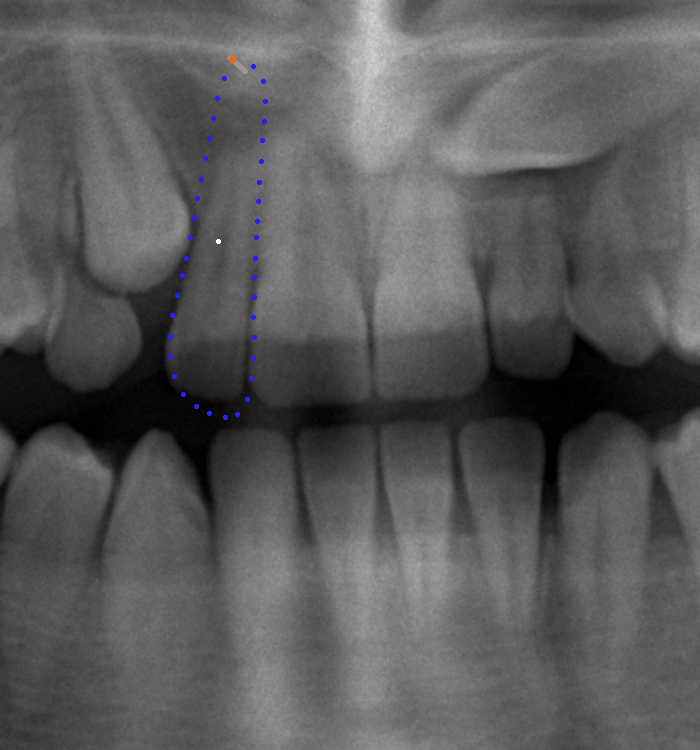
\includegraphics[width=\linewidth]{cropped1}
        \caption{Fitting of the midel into the tooth box}
        \label{fig:fitting1}
    \end{subfigure}
    \begin{subfigure}[b]{0.45\textwidth}
        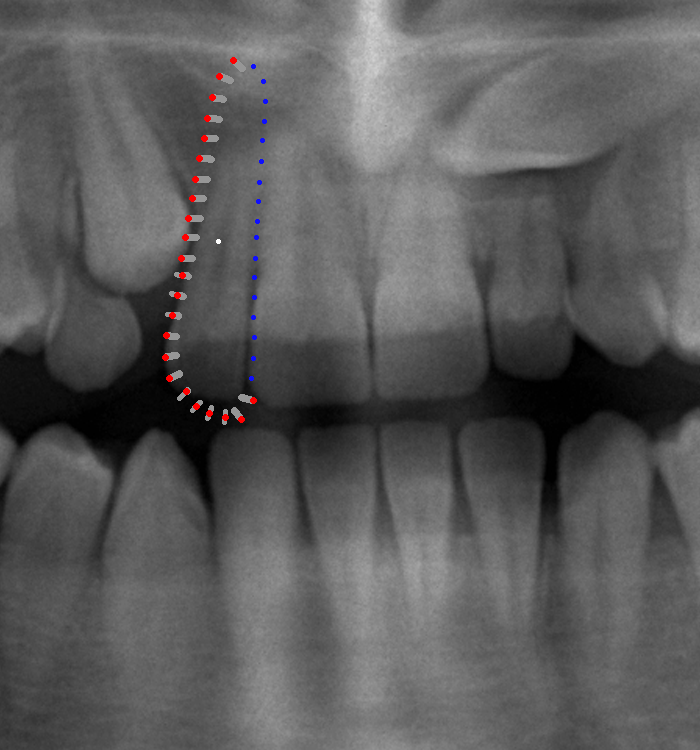
\includegraphics[width=\linewidth]{modelling} 
        \caption{Parsing the model to improve accuracy}
        \label{fig:fitting2}
    \end{subfigure}
    \caption{Steps while fitting the model over the image}
    \label{fig:fitting}
\end{figure}

\section{Evaluation and final considerations}\label{sec:evaluation}
In order to evaluate the obtained result, two error estimations are considered.

The first value we are computing is the Mean Squared Error. This represents the quadratic distance from the obtained model and the original landmarks. It is computed both for the \textit{x} and \textit{y} axis for every sample of which we have the corresponding landmarks. \\
The Mean Squared Error for each incisor is computed as: 
\begin{align}
   MSEx = \frac{1}{n_{teeth}} \sum_{i=1}^{n_{teeth}} \frac{1}{n_{lm}} \sum_{i=1}^{n_{lm}}(Xe_i - Xl_i)^2
\end{align}
\begin{align}
   MSEy = \frac{1}{n_{teeth}} \sum_{i=1}^{n_{teeth}} \frac{1}{n_{lm}} \sum_{i=1}^{n_{lm}}(Ye_i - Yl_i)^2
\end{align}
The second value we are computing is the Mean Absolute Error. It represents the absolute value of the difference between the estimated landmarks and the original ones. It is computed both for the \textit{x} and \textit{y} axis for every sample of which we have the corresponding landmarks. \\
The Mean Absolute Error is computed as: 
\begin{align}
    MAEx = \frac{1}{n_{teeth}} \sum_{i=1}^{n_{teeth}} \frac{1}{n_{lm}} \sum_{i=1}^{n_{lm}}|(Xe_i - Xl_i)|
\end{align}
\begin{align}
    MAEy = \frac{1}{n_{teeth}} \sum_{i=1}^{n_{teeth}} \frac{1}{n_{lm}} \sum_{i=1}^{n_{lm}}|(Ye_i - Yl_i)|
\end{align}
From the Mean Absolute Error it is possible to compute an estimation of the percentage error made with respect to the image dimensions. This can give an idea of how big the error is compared to the image resolution. 
To compute this value, the Mean Absolute Error needs to be divided consecutively by the image width , and the image height, and then multiplied by 100.

The algorithm has been tested using Leave one out Cross Validation on the data set containing 14 annotated radiographs. Therefore, the teeth models are build over the 13 images selected for testing while one is kept for testing. 

\begin{table}[h]
    \centering
    \begin{tabular}{c||c|c|c|c|}
    & \textbf{MSEx} & \textbf{MSEy} & \textbf{MAEx} & \textbf{MAEy} \\
    \hline \hline
    \textbf{1} & 2052.93 & 2255.69 & 10.04 & 6.10\\ \hline
    \textbf{2} & 309.05 & 392.54 & 0.97 & 1.12\\ \hline
    \textbf{3} & 335.12 & 1037.68 & 0.45 & 1.74\\ \hline
    \textbf{4} & 259.79 & 409.60 & 1.10 & 0.83\\ \hline
    \textbf{5} & 3475.37 & 1712.84 & 10.31 & 2.31\\ \hline
    \textbf{6} & 3042.80 & 1004.48 & 7.76 & 4.18\\ \hline
    \textbf{7} & 244.44 & 405.18 & 2.71 & 0.49\\ \hline
    \textbf{8} & 286.43 & 10644.19 & 0.71 & 10.59\\ \hline
    \textbf{9} & 4164.56 & 1980.69 & 11.35 & 2.51\\ \hline
    \textbf{10} & 4063.35 & 206.04 & 0.77 & 0.38\\ \hline
    \textbf{11} & 2155.47 & 512.22 & 2.19 & 2.34\\ \hline
    \textbf{12} & 2956.24 & 4429.92 & 10.85 & 7.74\\ \hline
    \textbf{13} & 186.61 & 205.67 & 1.85 & 2.24\\ \hline
    \textbf{14} & 150.68 & 425.43 & 0.71 & 1.30\\
    \hline
    \end{tabular}
    \caption{Results from the leave-one-out-testing. On the left the left out sample, in the first two columns the Mean Squared Error, in the last ones the Mean Absolute Error}
    \label{table:leaveoneout}
\end{table}
We can see, observing the results presented in Table \ref{table:leaveoneout}, that the errors have similar values. 
This proves that we have a stable model, which gives reliable results, having similar performance for every image. When the teeth on the radiographs are shifted to the side or have unusual orientations, the model can not fit them perfectly since the edges are not at the positions where they are expected to be. 

We can observe that the accuracy of the hand drawn boxes in the training has a significant affect on the outcome of the estimation. Based on these error indexes and intermediate results, we can infer that the estimated position of the incisors in the radiographs is mainly affected by the box fitting. \\
In addition, unusual teeth positions, caused for example by a bad accuracy when the radiograph itself was take, might affect the model as well. \\
Finally, we think that a larger training set could further improve the accuracy of the results. 

\begin{figure}[htp]
    \centering
    \begin{subfigure}[b]{0.45\textwidth}
        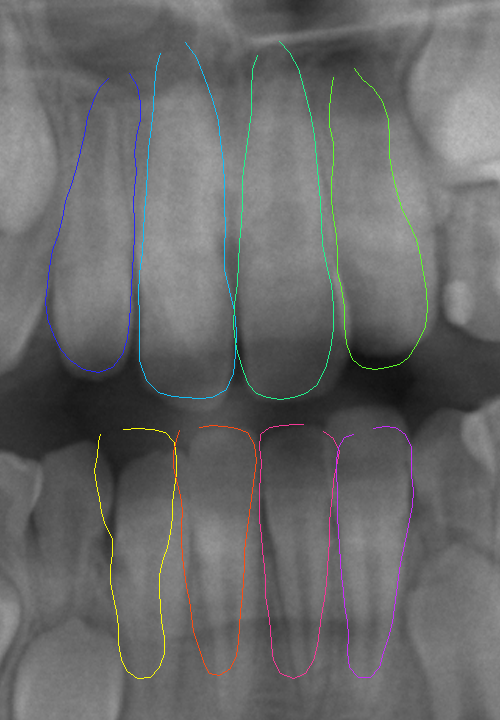
\includegraphics[width=\linewidth,height=7cm]{finalresult14test}
        \caption{Best results - Radiograph 14}
        \label{fig:bestresult}
    \end{subfigure}
    \begin{subfigure}[b]{0.45\textwidth}
        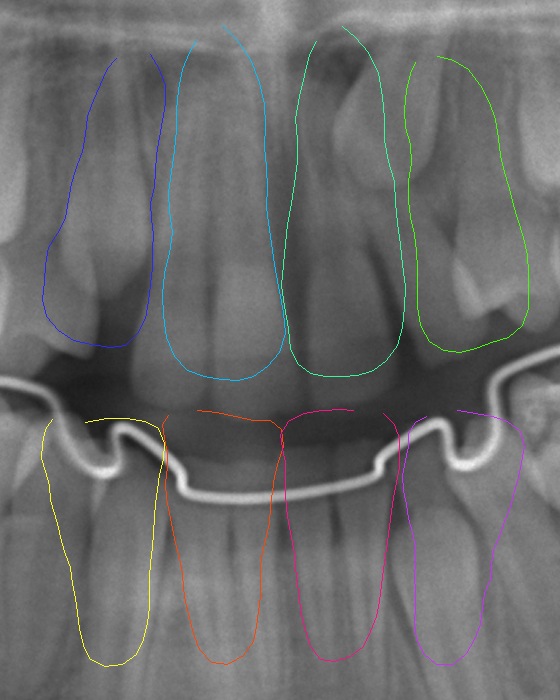
\includegraphics[width=\linewidth,height=7cm]{finalresult09test} 
        \caption{Worst results - Radiograph 9}
        \label{fig:worstresult}
    \end{subfigure}
    \caption{}
    \label{fig:bestandworst}
\end{figure}

The cause of the bad performance on the radiograph on Figure \ref{fig:worstresult} is the presence of the line with high intensity (probably braces). This is because the ground truth for the best fitting boxes is based on the pixel intensity inside the selected window. This leads to the wrong estimation of the best fitting box, returning the wrong image segment. Since the box is not the right dimension (too big) and we split it in four even parts to find the incisors, it can not detect them accurately.\\
When comparing the results from the hand drawn boxes and the estimated boxes, we can draw the same conclusion. There is a strong correlation between the image quality, estimated boxes and the performance of the algorithm. (Figure \ref{comp14} and Figure \ref{comp9})

\begin{figure}[h] 
    \centering
    \subcaptionbox{Radiograph 14
    \label{comp14}}{%
        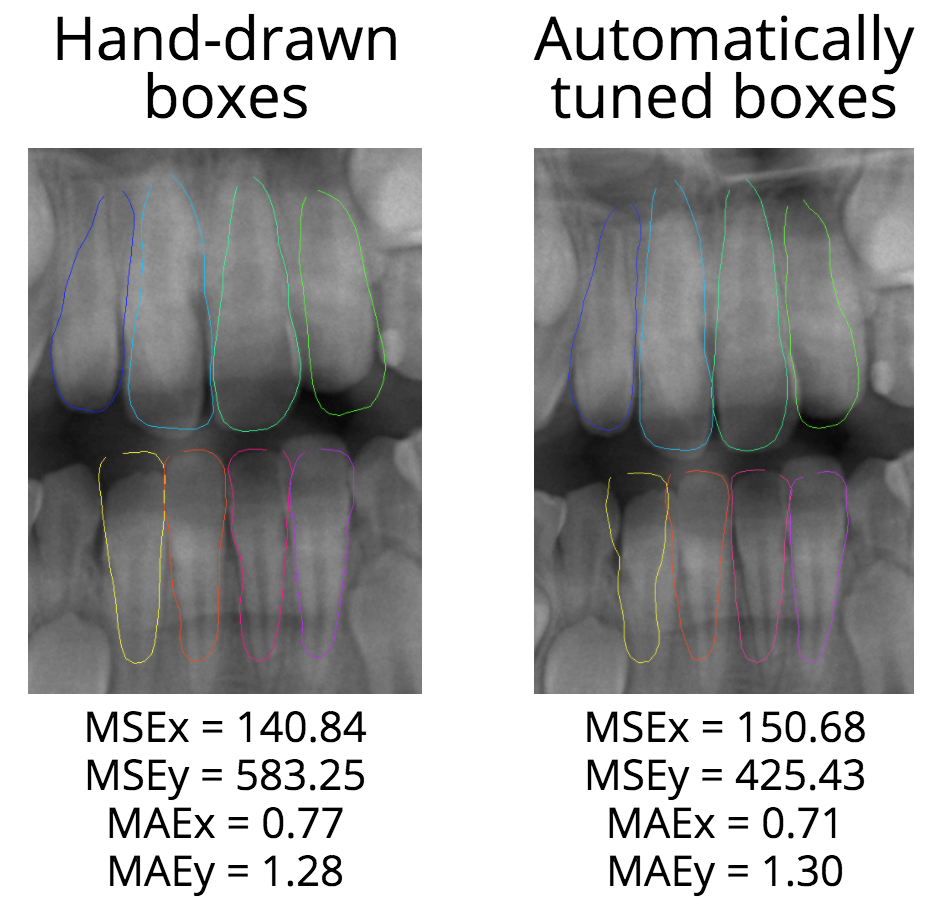
\includegraphics[width=0.8\textwidth]{r12}%
    }\par\medskip
    \subcaptionbox{Radiograph 9
    \label{comp9}}{%
        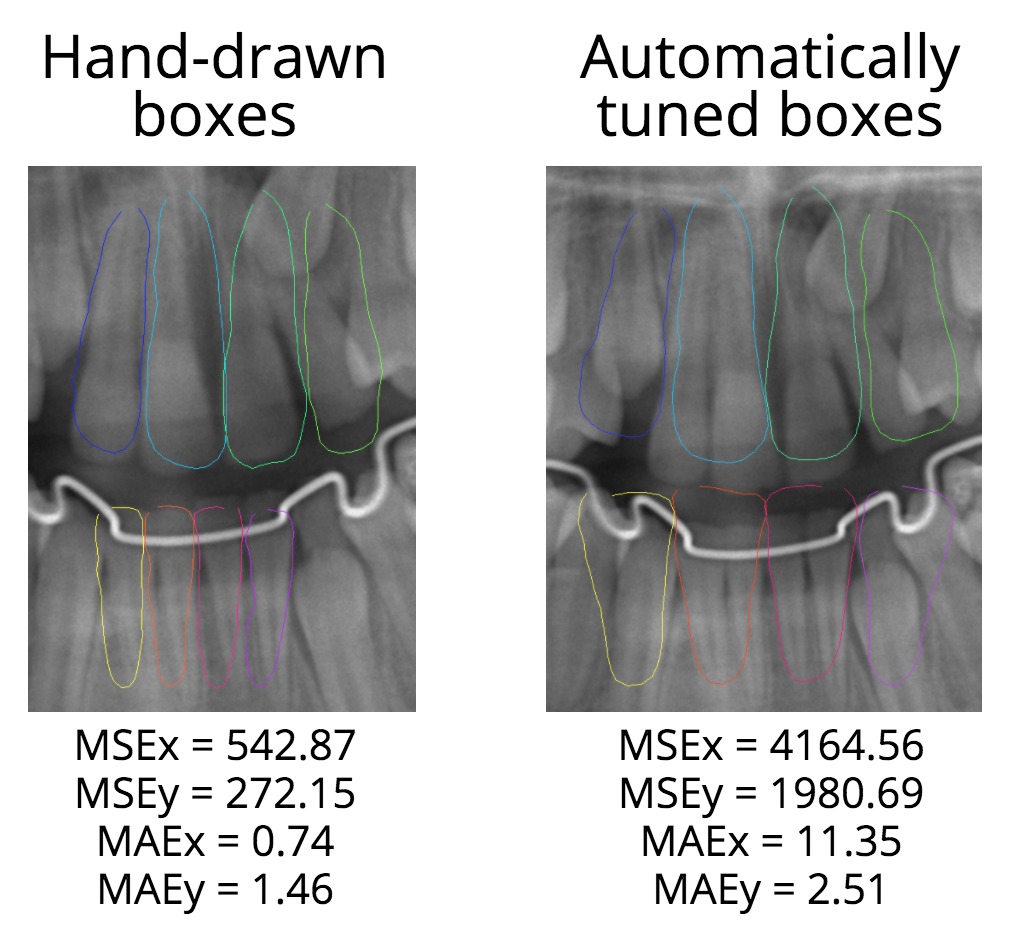
\includegraphics[width=0.8\textwidth]{r9}%
    }\par\medskip        
    \caption{Comparing results from hand drawn boxes and estimated boxes}
    \label{fig:compareboxes}
\end{figure}

\clearpage
\begin{thebibliography}{99}
    
    \bibitem{cootes}Cootes, Tim, E. Baldock, and J. Graham. "An introduction to active shape models." \textit{Image processing and analysis} (2000): 223-248.
    
    \bibitem{cootes2}Cootes, Timothy F., et al. "Active shape models-their training and application." \textit{Computer vision and image understanding} 61.1 (1995): 38-59.
    
    \bibitem{blanz}Blanz, Volker, et al. "A statistical method for robust 3D surface reconstruction from sparse data." \textit{3D Data Processing, Visualization and Transmission, 2004. 3DPVT 2004. Proceedings. 2nd International Symposium on.} IEEE, 2004.
    
    \bibitem{ahmad}Ahmad, Siti Arpah Bt, et al. "Utilizing contrast enhancement algorithms (CEAs) in identification of dental abnormalities." \textit{Technological Advances in Electrical, Electronics and Computer Engineering (TAEECE), 2013 International Conference on.} IEEE, 2013.
    
    \bibitem{paris}Paris, S., Kornprobst, P., Tumblin, J. and Durand, F., 2007, August. "A gentle introduction to bilateral filtering and its applications." In \textit{ACM SIGGRAPH 2007 courses} (p. 1). ACM.
    
    \bibitem{huang}R.-Y. Huang, L.-R. Dung, C.-F. Chu, and Y.-Y.Wu. "Noise removal and contrast enhancement for x-ray images." \textit{Journal of Biomedical Engineering and Medical Imaging}, 3(1):56, 2016.
11
    
    \bibitem{paper4}"Model reconstruction". Computer Vision [H02K5a], KU Leuven 
    
    %\bibitem{cohnen} 
    %M Cohnen, J Kemper, O M ̈obes, J Pawelzik, and U M ̈odder. Radiation dose in dental radiology.,
    %\textit{European radiology}. 
    %12(3):634–637, 2002
    % 
    %\bibitem{anil} 
    %Anil K Jain and Hong Chen. Matching of dental x-ray images for human identification.,
    %\\\textit{37(7):1519–1532, 2004.}

\end{thebibliography}

\end{document}